\documentclass[12pt,a4paper]{article}

\usepackage[margin=1in]{geometry}
\usepackage{amsmath, amssymb, amsthm}
\usepackage{enumitem}
\usepackage{booktabs}
\usepackage{tikz}
\usetikzlibrary{arrows.meta, positioning}

\setlength{\parindent}{0pt}
\setlength{\parskip}{6pt}

\newtheoremstyle{notestyle}
  {8pt}
  {8pt}
  {\normalfont}
  {}
  {\bfseries}
  {.}
  {0.5em}
  {}

\theoremstyle{notestyle}
\newtheorem{definition}{Definition}
\newtheorem{example}{Example}

\newenvironment{answer}
{\par\textbf{Answer.}\ }
{\hfill$\square$\par}

\newcommand{\Prob}{\mathbb{P}}

\title{\textbf{Supplementary Notes: Recurrent and Transient States}}
\author{MA4034: Time Series and Stochastic Processes}
\date{}

\begin{document}
\maketitle

\section{Main Idea}

In a Markov chain, a state is called \textbf{recurrent} if, once we visit that state, we are guaranteed to return to it eventually. A state is called \textbf{transient} if there is a chance that, after leaving it, we will never return.

\begin{definition}[First Return Time]
For a state $i$, define
\[
\tau_i=\min\{n\geq 1:X_n=i\}.
\]
This is the first time the chain returns to state $i$ after starting from $i$. If the chain never returns to $i$, then
\[
\tau_i=\infty.
\]
\end{definition}

\begin{definition}[Recurrent State]
A state $i$ is \textbf{recurrent} if
\[
\Prob_i(\tau_i<\infty)=1.
\]
That is, starting from state $i$, the chain returns to $i$ eventually with probability 1.
\end{definition}

\begin{definition}[Transient State]
A state $i$ is \textbf{transient} if
\[
\Prob_i(\tau_i<\infty)<1.
\]
That is, starting from state $i$, there is a positive probability that the chain will never return to $i$.
\end{definition}

\textbf{Simple analogy.} A recurrent state is like a home that you are guaranteed to visit again. A transient state is like a place you may pass through once and never see again.

\section{How to Identify Recurrent and Transient States from a Diagram}

The easiest way is to study the transition diagram.

\begin{itemize}[leftmargin=1.2cm]
    \item If a state leads to a closed group of states and cannot be reached again, it is usually transient.
    \item If a state belongs to a closed communicating class, it is recurrent.
    \item An absorbing state is recurrent.
    \item In a finite Markov chain, every closed communicating class consists of recurrent states.
\end{itemize}

\begin{definition}[Closed Class]
A set of states $C$ is called \textbf{closed} if, once the chain enters $C$, it cannot leave $C$.
\end{definition}

\section{Transition Diagrams}

\subsection{Diagram 1: Absorbing State}

\begin{center}
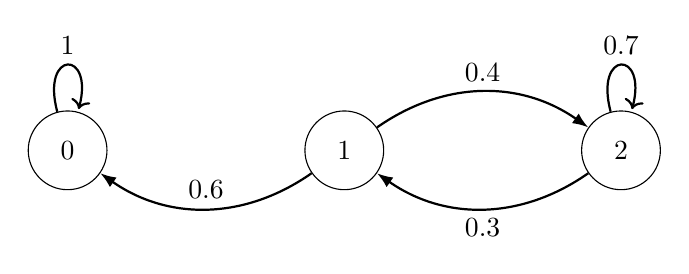
\begin{tikzpicture}[
  state/.style={circle, draw, minimum size=10mm},
  edge/.style={-{Latex[length=2mm]}, thick},
  bend angle=35
]
\node[state] (0) {$0$};
\node[state, right=25mm of 0] (1) {$1$};
\node[state, right=25mm of 1] (2) {$2$};

\draw[edge] (0) edge[loop above] node {$1$} (0);
\draw[edge] (1) edge[bend left] node[above] {$0.6$} (0);
\draw[edge] (1) edge[bend left] node[above] {$0.4$} (2);
\draw[edge] (2) edge[loop above] node {$0.7$} (2);
\draw[edge] (2) edge[bend left] node[below] {$0.3$} (1);
\end{tikzpicture}
\end{center}

Here state $0$ is absorbing. Once the chain enters state $0$, it stays there forever.

\begin{itemize}[leftmargin=1.2cm]
    \item State $0$ is recurrent.
    \item States $1$ and $2$ are transient because the chain may eventually enter state $0$ and never return to them.
\end{itemize}

\subsection{Diagram 2: Closed Communicating Class}

\begin{center}
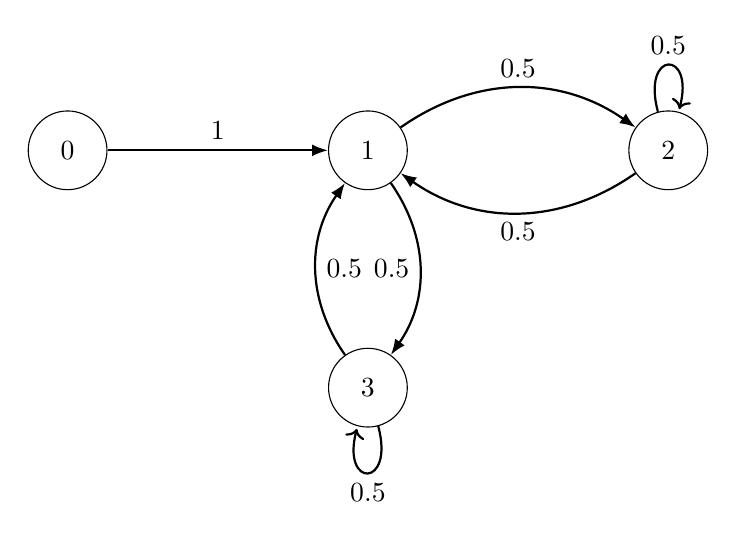
\begin{tikzpicture}[
  state/.style={circle, draw, minimum size=10mm},
  edge/.style={-{Latex[length=2mm]}, thick},
  bend angle=35
]
\node[state] (0) {$0$};
\node[state, right=28mm of 0] (1) {$1$};
\node[state, right=28mm of 1] (2) {$2$};
\node[state, below=20mm of 1] (3) {$3$};

\draw[edge] (0) -- node[above] {$1$} (1);
\draw[edge] (1) edge[bend left] node[above] {$0.5$} (2);
\draw[edge] (2) edge[bend left] node[below] {$0.5$} (1);
\draw[edge] (1) edge[bend left] node[left] {$0.5$} (3);
\draw[edge] (3) edge[bend left] node[right] {$0.5$} (1);
\draw[edge] (2) edge[loop above] node {$0.5$} (2);
\draw[edge] (3) edge[loop below] node {$0.5$} (3);
\end{tikzpicture}
\end{center}

The set
\[
\{1,2,3\}
\]
is closed and communicating: once the chain enters it, it cannot leave, and all three states can reach each other.

\begin{itemize}[leftmargin=1.2cm]
    \item State $0$ is transient because once it moves to state $1$, it can never return to $0$.
    \item States $1,2,3$ are recurrent because they form a closed communicating class.
\end{itemize}

\subsection{Diagram 3: Irreducible Finite Chain}

\begin{center}
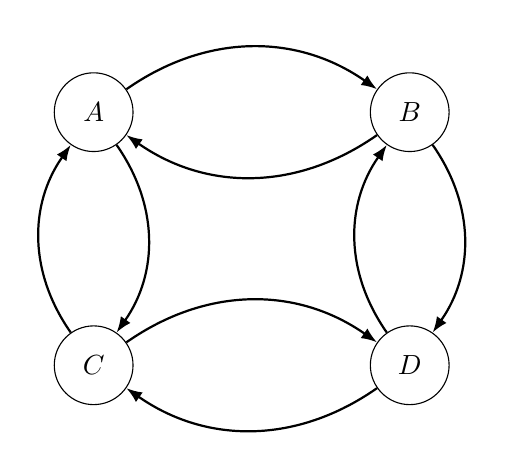
\begin{tikzpicture}[
  state/.style={circle, draw, minimum size=10mm},
  edge/.style={-{Latex[length=2mm]}, thick},
  bend angle=35
]
\node[state] (A) {$A$};
\node[state, right=30mm of A] (B) {$B$};
\node[state, below=22mm of A] (C) {$C$};
\node[state, below=22mm of B] (D) {$D$};

\draw[edge] (A) edge[bend left] node[above] {} (B);
\draw[edge] (B) edge[bend left] node[below] {} (A);
\draw[edge] (A) edge[bend left] node[left] {} (C);
\draw[edge] (C) edge[bend left] node[right] {} (A);
\draw[edge] (B) edge[bend left] node[right] {} (D);
\draw[edge] (D) edge[bend left] node[left] {} (B);
\draw[edge] (C) edge[bend left] node[below] {} (D);
\draw[edge] (D) edge[bend left] node[above] {} (C);
\end{tikzpicture}
\end{center}

All states communicate with each other. The chain is finite and irreducible.

\begin{itemize}[leftmargin=1.2cm]
    \item States $A,B,C,D$ are all recurrent.
\end{itemize}

\subsection{Diagram 4: One-Way Escape}

\begin{center}
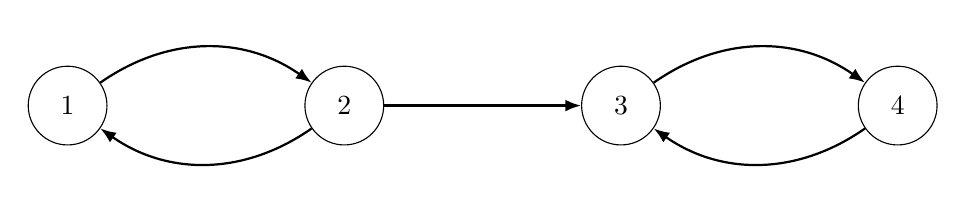
\begin{tikzpicture}[
  state/.style={circle, draw, minimum size=10mm},
  edge/.style={-{Latex[length=2mm]}, thick},
  bend angle=35
]
\node[state] (1) {$1$};
\node[state, right=25mm of 1] (2) {$2$};
\node[state, right=25mm of 2] (3) {$3$};
\node[state, right=25mm of 3] (4) {$4$};

\draw[edge] (1) edge[bend left] node[above] {} (2);
\draw[edge] (2) edge[bend left] node[below] {} (1);
\draw[edge] (2) -- node[above] {} (3);
\draw[edge] (3) edge[bend left] node[above] {} (4);
\draw[edge] (4) edge[bend left] node[below] {} (3);
\end{tikzpicture}
\end{center}

The set $\{3,4\}$ is closed. Once the chain enters $\{3,4\}$, it cannot return to $\{1,2\}$.

\begin{itemize}[leftmargin=1.2cm]
    \item States $1$ and $2$ are transient.
    \item States $3$ and $4$ are recurrent.
\end{itemize}

\section{Important Corollary: Irreducible Chains}

\[
\boxed{\text{In an irreducible Markov chain, either all states are recurrent or all states are transient.}}
\]

This statement is very important. It says that in an irreducible chain, recurrence and transience are not properties of isolated states. They become properties of the whole chain.

Recall that a Markov chain is \textbf{irreducible} if every state can communicate with every other state. That means for any two states $i$ and $j$,
\[
i\to j
\qquad\text{and}\qquad
j\to i.
\]

\subsection{Why This Happens}

Suppose state $i$ is recurrent, and state $j$ communicates with $i$.

Since $i\to j$, there is a positive probability of going from $i$ to $j$. Since $j\to i$, there is also a positive probability of coming back from $j$ to $i$.

If state $i$ is recurrent, the chain keeps returning to $i$. Every time it returns to $i$, it gets another chance to go to $j$. Because this chance keeps repeating, state $j$ must also be visited again and again. Therefore $j$ is recurrent too.

Similarly, if one state is transient in an irreducible chain, then every state must be transient. If some other state were recurrent, then by communication it would force the first state to be recurrent as well, which is a contradiction.

\textbf{Simple analogy.} Imagine all states are rooms connected by two-way doors. If one room is guaranteed to be revisited forever, then because every room is reachable from every other room, the whole connected building is revisited forever. But if one room can be permanently left behind, then the same risk applies to all rooms in that connected system.

\subsection{Diagram A: Irreducible Finite Chain}

\begin{center}
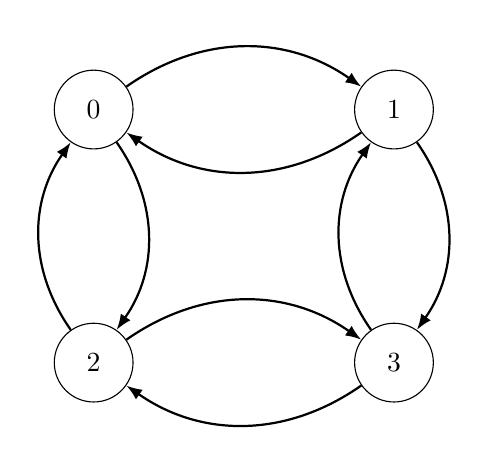
\begin{tikzpicture}[
  state/.style={circle, draw, minimum size=10mm},
  edge/.style={-{Latex[length=2mm]}, thick},
  bend angle=35
]
\node[state] (0) {$0$};
\node[state, right=28mm of 0] (1) {$1$};
\node[state, below=22mm of 0] (2) {$2$};
\node[state, below=22mm of 1] (3) {$3$};

\draw[edge] (0) edge[bend left] node[above] {} (1);
\draw[edge] (1) edge[bend left] node[below] {} (0);
\draw[edge] (0) edge[bend left] node[left] {} (2);
\draw[edge] (2) edge[bend left] node[right] {} (0);
\draw[edge] (1) edge[bend left] node[right] {} (3);
\draw[edge] (3) edge[bend left] node[left] {} (1);
\draw[edge] (2) edge[bend left] node[below] {} (3);
\draw[edge] (3) edge[bend left] node[above] {} (2);
\end{tikzpicture}
\end{center}

In this diagram, every state can reach every other state. Therefore the chain is irreducible.

Since the state space is finite, the chain cannot keep escaping to new states forever. It must keep revisiting states. In a finite irreducible chain, all states are recurrent.

\[
\boxed{\text{All states }0,1,2,3\text{ are recurrent.}}
\]

\subsection{Diagram B: Why Mixed Behaviour is Not Possible in an Irreducible Chain}

The following diagram is \textbf{not} irreducible:

\begin{center}
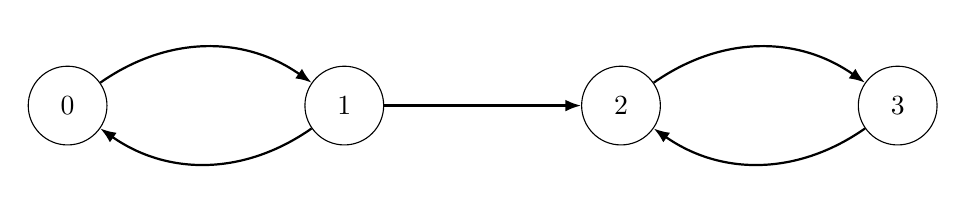
\begin{tikzpicture}[
  state/.style={circle, draw, minimum size=10mm},
  edge/.style={-{Latex[length=2mm]}, thick},
  bend angle=35
]
\node[state] (0) {$0$};
\node[state, right=25mm of 0] (1) {$1$};
\node[state, right=25mm of 1] (2) {$2$};
\node[state, right=25mm of 2] (3) {$3$};

\draw[edge] (0) edge[bend left] node[above] {} (1);
\draw[edge] (1) edge[bend left] node[below] {} (0);
\draw[edge] (1) -- node[above] {} (2);
\draw[edge] (2) edge[bend left] node[above] {} (3);
\draw[edge] (3) edge[bend left] node[below] {} (2);
\end{tikzpicture}
\end{center}

Here states $0$ and $1$ can communicate with each other, and states $2$ and $3$ can communicate with each other. But once the chain moves from state $1$ to state $2$, it cannot go back to states $0$ or $1$.

So the chain can have mixed behaviour:
\[
\{0,1\}\text{ transient},\qquad \{2,3\}\text{ recurrent}.
\]

This mixed behaviour is possible only because the chain is reducible. If the chain were irreducible, there would also need to be a path from $\{2,3\}$ back to $\{0,1\}$.

\subsection{Diagram C: Irreducible Infinite Chain}

Irreducible chains do not always have to be recurrent. Infinite irreducible chains can be transient.

For example, imagine a random walk on all integers:
\[
\cdots,-2,-1,0,1,2,\cdots
\]
where the chain can move left or right from every state.

\begin{center}
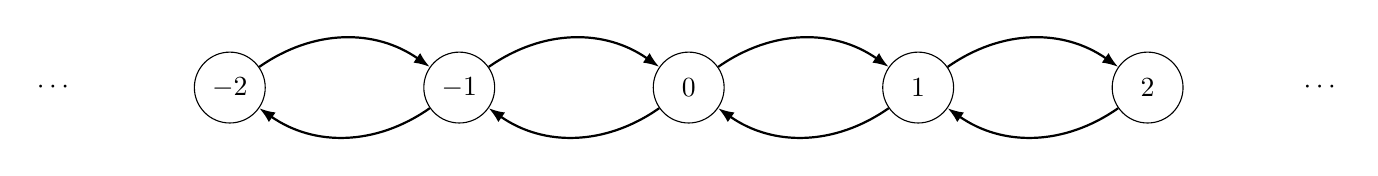
\begin{tikzpicture}[
  state/.style={circle, draw, minimum size=9mm},
  edge/.style={-{Latex[length=2mm]}, thick},
  bend angle=35
]
\node (leftdots) {$\cdots$};
\node[state, right=14mm of leftdots] (m2) {$-2$};
\node[state, right=20mm of m2] (m1) {$-1$};
\node[state, right=20mm of m1] (z) {$0$};
\node[state, right=20mm of z] (p1) {$1$};
\node[state, right=20mm of p1] (p2) {$2$};
\node[right=14mm of p2] (rightdots) {$\cdots$};

\draw[edge] (m2) edge[bend left] (m1);
\draw[edge] (m1) edge[bend left] (m2);
\draw[edge] (m1) edge[bend left] (z);
\draw[edge] (z) edge[bend left] (m1);
\draw[edge] (z) edge[bend left] (p1);
\draw[edge] (p1) edge[bend left] (z);
\draw[edge] (p1) edge[bend left] (p2);
\draw[edge] (p2) edge[bend left] (p1);
\end{tikzpicture}
\end{center}

Every state can reach every other state, so this type of chain is irreducible.

Depending on the transition probabilities and dimension of the random walk, such an infinite irreducible chain may be recurrent or transient. But the corollary says it cannot be mixed:

\[
\boxed{\text{If one state is recurrent, all states are recurrent.}}
\]
\[
\boxed{\text{If one state is transient, all states are transient.}}
\]

\subsection{Key Lesson}

For an irreducible Markov chain, we do not classify states one by one. We classify the entire chain:

\[
\text{irreducible chain}
\quad\Longrightarrow\quad
\begin{cases}
\text{all states recurrent},\\
\text{or}\\
\text{all states transient}.
\end{cases}
\]

\section{Practice Questions}

\begin{enumerate}[label=\textbf{Q\arabic*.}, leftmargin=1.2cm]
    \item Consider the transition diagram
    \[
    0\to 1,\qquad 1\to 2,\qquad 2\to 2.
    \]
    Identify the recurrent and transient states.

    \item Consider a Markov chain with transition matrix
    \[
    P=
    \begin{pmatrix}
    1 & 0 & 0\\
    0.4 & 0.2 & 0.4\\
    0 & 0 & 1
    \end{pmatrix}.
    \]
    Identify the recurrent and transient states.

    \item Consider the transition diagram
    \[
    1\leftrightarrow 2,\qquad 2\to 3,\qquad 3\leftrightarrow 4.
    \]
    There is no arrow from states $3$ or $4$ back to states $1$ or $2$. Identify the recurrent and transient states.

    \item Consider a finite irreducible Markov chain with states
    \[
    S=\{A,B,C\}.
    \]
    What can you say about recurrence or transience of the states?

    \item Consider the Markov chain with transition matrix
    \[
    P=
    \begin{pmatrix}
    0.5 & 0.5 & 0\\
    0.5 & 0.5 & 0\\
    0.2 & 0.3 & 0.5
    \end{pmatrix}.
    \]
    Identify the recurrent and transient states.

    \item Consider the Markov chain with transition matrix
    \[
    P=
    \begin{pmatrix}
    0 & 1 & 0 & 0\\
    1 & 0 & 0 & 0\\
    0 & 0.5 & 0 & 0.5\\
    0 & 0 & 1 & 0
    \end{pmatrix}.
    \]
    Identify the recurrent and transient states.

    \item A student says: ``If a state has a self-loop, then it is always recurrent.'' Is this statement true? Explain using an example.

    \item A student says: ``If a state is absorbing, then it is recurrent.'' Is this statement true? Explain.
\end{enumerate}

\section{Answers}

\subsection*{Answer 1}

The chain is
\[
0\to 1,\qquad 1\to 2,\qquad 2\to 2.
\]

State $2$ is absorbing because once the chain reaches state $2$, it stays there. Therefore state $2$ is recurrent.

State $0$ moves to state $1$ and cannot return to state $0$. Hence state $0$ is transient.

State $1$ moves to state $2$ and cannot return to state $1$. Hence state $1$ is transient.

Therefore:
\[
\boxed{\text{Recurrent: } \{2\}}
\]
and
\[
\boxed{\text{Transient: } \{0,1\}.}
\]

\subsection*{Answer 2}

The matrix is
\[
P=
\begin{pmatrix}
1 & 0 & 0\\
0.4 & 0.2 & 0.4\\
0 & 0 & 1
\end{pmatrix}.
\]

State $0$ is absorbing because
\[
p_{00}=1.
\]
Thus state $0$ is recurrent.

State $2$ is also absorbing because
\[
p_{22}=1.
\]
Thus state $2$ is recurrent.

From state $1$, the chain can move to state $0$ or state $2$. Once it reaches either state $0$ or state $2$, it cannot return to state $1$. Therefore state $1$ is transient.

Thus:
\[
\boxed{\text{Recurrent: } \{0,2\}}
\]
and
\[
\boxed{\text{Transient: } \{1\}.}
\]

\subsection*{Answer 3}

States $1$ and $2$ communicate with each other. States $3$ and $4$ also communicate with each other.

However, there is a one-way path from state $2$ to state $3$, and there is no path from states $3$ or $4$ back to states $1$ or $2$.

Therefore, once the chain enters the class
\[
\{3,4\},
\]
it cannot leave. Hence $\{3,4\}$ is a closed communicating class, so states $3$ and $4$ are recurrent.

States $1$ and $2$ are transient because the chain may leave them and enter $\{3,4\}$ forever.

Thus:
\[
\boxed{\text{Recurrent: } \{3,4\}}
\]
and
\[
\boxed{\text{Transient: } \{1,2\}.}
\]

\subsection*{Answer 4}

In a finite irreducible Markov chain, all states communicate with each other. Since the chain is finite, there must be at least one recurrent class. Because the chain is irreducible, the whole state space is one communicating class.

Therefore all states are recurrent.

Thus:
\[
\boxed{\text{Recurrent: } \{A,B,C\}}
\]
and
\[
\boxed{\text{Transient: none}.}
\]

\subsection*{Answer 5}

The matrix is
\[
P=
\begin{pmatrix}
0.5 & 0.5 & 0\\
0.5 & 0.5 & 0\\
0.2 & 0.3 & 0.5
\end{pmatrix}.
\]

States $0$ and $1$ communicate with each other, and once the chain is in the set
\[
\{0,1\},
\]
it cannot move to state $2$ because
\[
p_{02}=0,\qquad p_{12}=0.
\]
So $\{0,1\}$ is a closed communicating class. Therefore states $0$ and $1$ are recurrent.

From state $2$, there is a positive probability of moving to state $0$ or state $1$. Once the chain reaches $\{0,1\}$, it cannot return to state $2$. Therefore state $2$ is transient.

Thus:
\[
\boxed{\text{Recurrent: } \{0,1\}}
\]
and
\[
\boxed{\text{Transient: } \{2\}.}
\]

\subsection*{Answer 6}

The transition matrix is
\[
P=
\begin{pmatrix}
0 & 1 & 0 & 0\\
1 & 0 & 0 & 0\\
0 & 0.5 & 0 & 0.5\\
0 & 0 & 1 & 0
\end{pmatrix}.
\]

States $0$ and $1$ communicate:
\[
0\to 1,\qquad 1\to 0.
\]
Also, once the chain enters $\{0,1\}$, it cannot leave. Hence $\{0,1\}$ is a closed communicating class, so states $0$ and $1$ are recurrent.

State $2$ can move to state $1$ with probability $0.5$. Once the chain reaches state $1$, it is trapped in the closed class $\{0,1\}$ and cannot return to state $2$. Therefore state $2$ is transient.

State $3$ moves to state $2$, and then the chain may enter $\{0,1\}$ and never return to state $3$. Therefore state $3$ is transient.

Thus:
\[
\boxed{\text{Recurrent: } \{0,1\}}
\]
and
\[
\boxed{\text{Transient: } \{2,3\}.}
\]

\subsection*{Answer 7}

The statement is false. A self-loop alone does not guarantee recurrence.

For example, consider
\[
P=
\begin{pmatrix}
0.5 & 0.5\\
0 & 1
\end{pmatrix}.
\]
State $0$ has a self-loop because
\[
p_{00}=0.5.
\]
However, from state $0$, the chain can move to state $1$ with probability $0.5$. Once it reaches state $1$, it stays there forever and cannot return to state $0$.

Therefore state $0$ is transient even though it has a self-loop.

\subsection*{Answer 8}

The statement is true. If a state $i$ is absorbing, then
\[
p_{ii}=1.
\]
This means that once the chain enters state $i$, it remains there forever.

Therefore, starting from state $i$, the chain returns to state $i$ at the next step with probability 1:
\[
\Prob_i(\tau_i<\infty)=1.
\]
Hence every absorbing state is recurrent.

\end{document}
